\documentclass[../notes.tex]{subfiles}

\pagestyle{main}
\renewcommand{\chaptermark}[1]{\markboth{\chaptername\ \thechapter\ (#1)}{}}
\setcounter{chapter}{8}

\begin{document}




\chapter{Particle Physics}
\section{Spin in a Magnetic Field}
\begin{itemize}
    \item \marginnote{2/26:}Today's goal: Spin in a magnetic field.
    \item Review.
    \begin{itemize}
        \item We describe spin as an intrinsic angular momentum.
        \item It has three components $\hat{S}_x,\hat{S}_y,\hat{S}_z$ that don't commute with each other:
        \begin{equation*}
            [\hat{S}_x,\hat{S}_y] = i\hbar\hat{S}_z
        \end{equation*}
        \item The spin operators obey the usual rules of angular momentum, i.e., we can define a state with a definite value of spin squared and direction.
        \begin{align*}
            \hat{\vec{S}}{\,}^2\ket{s,m_s} &= \hbar^2s(s+1)\ket{s,m_s}\\
            \hat{S}_z\ket{s,m_s} &= \hbar m_s\ket{s,m_s}
        \end{align*}
        \item We discovered that the values of $s$ can take half-integer values.
        \begin{itemize}
            \item There are $2s+1$ states for a given $s$, related to the fact that we can have differnt projections of the spin in the $z$-direction indexed by values $-s\leq m_s\leq s$.
        \end{itemize}
        \item A particle moving in the hydrogen atom can only have $\pm 1/2$ states, called "spin up" or "spin down."
        \begin{itemize}
            \item This comes from the fact that in this space, a good representation of the spin operator is in terms of the Pauli matrices:
            \begin{align*}
                \hat{S}_z &= \frac{\hbar}{2}
                \begin{pmatrix}
                    1 & 0\\
                    0 & -1\\
                \end{pmatrix}&
                \hat{S}_x &= \frac{\hbar}{2}
                \begin{pmatrix}
                    0 & 1\\
                    1 & 0\\
                \end{pmatrix}&
                \hat{S}_y &= \frac{\hbar}{2}
                \begin{pmatrix}
                    0 & -i\\
                    i & 0\\
                \end{pmatrix}
            \end{align*}
            \begin{itemize}
                \item Observe that these are Hermitian matrices.
            \end{itemize}
        \end{itemize}
        \item It follows from the matrix definition that
        \begin{equation*}
            \hat{S}_i^2 = \frac{\hbar^2}{4}I
        \end{equation*}
        for $i=x,y,z$ and hence
        \begin{equation*}
            \hat{\vec{S}}{\,}^2 = \hat{S}_x^2+\hat{S}_y^2+\hat{S}_z^2
            = \frac{3\hbar^2}{4}I
        \end{equation*}
        \item If we perform a measurement of the spin in any direction, we always obtain $\pm\hbar/2$.
        \begin{itemize}
            \item This is because these are the eigenvalues of the spin operator (the observables).
        \end{itemize}
        \item An additional layer of formalism: Spinors.
        \item We defined $\chi_\pm$, which have the properties that
        \begin{align*}
            \hat{S}_z\chi_+ &= \frac{\hbar}{2}\chi_+&
            \hat{S}_z\chi_- &= -\frac{\hbar}{2}\chi_-
        \end{align*}
        \begin{itemize}
            \item We sometimes denote these eigenstates as $\chi_\pm^z$.
        \end{itemize}
        \item In the $x$-direction, we have
        \begin{align*}
            \chi_+^x &= \frac{1}{\sqrt{2}}
            \begin{pmatrix}
                1\\
                1\\
            \end{pmatrix}&
                \chi_-^x &= \frac{1}{\sqrt{2}}
                \begin{pmatrix}
                    1\\
                    -1\\
                \end{pmatrix}\\
            \hat{S}_z\chi_+^x &= \frac{\hbar}{2}\chi_+^x&
                \hat{S}_z\chi_-^x &= -\frac{\hbar}{2}\chi_-^x
        \end{align*}
        \item In the $y$-direction, we have
        \begin{align*}
            \chi_+^y &= \frac{1}{\sqrt{2}}
            \begin{pmatrix}
                1\\
                i\\
            \end{pmatrix}&
                \chi_-^y &= \frac{1}{\sqrt{2}}
                \begin{pmatrix}
                    1\\
                    -i\\
                \end{pmatrix}\\
            \hat{S}_z\chi_+^y &= \frac{\hbar}{2}\chi_+^y&
                \hat{S}_z\chi_-^y &= -\frac{\hbar}{2}\chi_-^y
        \end{align*}
        \item It follows from the normalization that
        \begin{equation*}
            |\chi_+|^2+|\chi_-|^2 = 1
        \end{equation*}
        and hence that $|\chi_+|^2$ is the probability of finding the part with spin up in $z$.
        \item We define the state
        \begin{equation*}
            \chi =
            \begin{pmatrix}
                \chi_+\\
                \chi_-\\
            \end{pmatrix}
        \end{equation*}
        and can find that
        \begin{equation*}
            \ev{\hat{S}_z}{\chi} = \frac{\hbar}{2}
            \begin{pmatrix}
                \chi_+^* & \chi_-^*\\
            \end{pmatrix}
            \begin{pmatrix}
                1 & 0\\
                0 & -1\\
            \end{pmatrix}
            \begin{pmatrix}
                \chi_+\\
                \chi_-\\
            \end{pmatrix}
            = \frac{\hbar}{2}\left( |\chi_+|^2-|\chi_-|^2 \right)
        \end{equation*}
        \item We can introduce coefficients such that
        \begin{equation*}
            \chi = c_+\chi_+^z+c_-\chi_-^z
            =
            \begin{pmatrix}
                c_+\\
                c_-\\
            \end{pmatrix}
            =:
            \begin{pmatrix}
                \chi_+\\
                \chi_-\\
            \end{pmatrix}
        \end{equation*}
        and
        \begin{equation*}
            \chi = d_+\chi_+^x+d_-\chi_-^x
            =:
            \begin{pmatrix}
                \chi_+\\
                \chi_-\\
            \end{pmatrix}
        \end{equation*}
        \item Then herein, $|d_\pm|^2$ is the probability of finding the particle with spin up or down in the $x$-direction.
        \item To find one of the two components of the spin eigenstate in a certain direction, take the inner product with the desired eigenstate.
        \begin{itemize}
            \item Examples:
            \begin{align*}
                \begin{pmatrix}
                    1 & 0\\
                \end{pmatrix}
                \begin{pmatrix}
                    \chi_+^z\\
                    \chi_-^z\\
                \end{pmatrix}
                &= c_+&
                \frac{1}{\sqrt{2}}
                \begin{pmatrix}
                    1 & 1\\
                \end{pmatrix}
                \begin{pmatrix}
                    \chi_+^x\\
                    \chi_-^x\\
                \end{pmatrix}
                &= d_+
            \end{align*}
            \item Essentially, we are making use of the following orthogonality relation.
            \begin{equation*}
                \chi_+^\dagger\chi = \chi_+^\dagger(d_+\chi_+^x+d_-\chi_-^x)
                = d_+\chi_+^\dagger\chi_++d_-\chi_+^\dagger\chi_-
                = d_+\cdot 1+d_-\cdot 0
                = d_+
            \end{equation*}
            \item This orthogonality relation is a specific case of the following, more general one.
            \begin{equation*}
                (\chi_+^i)^\dagger\chi_-^i = 0
            \end{equation*}
        \end{itemize}
        \item An explanation of the spinor entries.
        \begin{itemize}
            \item Since
            \begin{equation*}
                \ev{\hat{S}_z}{\tfrac{1}{2},\tfrac{1}{2}} = \frac{\hbar}{2}
            \end{equation*}
            and
            \begin{equation*}
                \ev{\hat{S}_x}{\tfrac{1}{2},\tfrac{1}{2}} = \frac{1}{2}\ev{(\hat{S}_++\hat{S}_-)}{\tfrac{1}{2},\tfrac{1}{2}}
                = 0
            \end{equation*}
            we have that the probability has to be spin up or down; it can't be side to side.
        \end{itemize}
    \end{itemize}
    \item We now begin on new content: A spin in a magnetic field.
    \begin{itemize}
        \item This is related to the interaction between two magnetic fields.
    \end{itemize}
    \item Recall that when a charged particle spins, it acquires a magnetic moment
    \begin{equation*}
        \vec{\mu} = \underbrace{\frac{qe}{2M}\cdot g}_\gamma\vec{S}
    \end{equation*}
    \begin{itemize}
        \item $g$ is called the \textbf{gyromagnetic factor}.
        \item At Fermilab, it was measured/computed to be
        \begin{equation*}
            g = 2+\frac{\alpha}{2\pi}+\cdots
        \end{equation*}
        where $\alpha$ is electromagnetic fine structure constant from the 2/16 lecture.
        \item Compute $g$ to $5^5$ decimal places via experiment, Dirac equation/relativity, quantum corrections.
        \item Kinoshita was a god of computation that made an error in this field and there's some politically incorrect story about that.
    \end{itemize}
    \item From here, we define the Hamiltonian
    \begin{equation*}
        \hat{H} = -\vec{\mu}\cdot\vec{B}-\frac{\hbar^2}{2M}\vec{\nabla}^2+V(\vec{r},t)
    \end{equation*}
    \item Now here, the eigenfunction is a spinor with two components, so we need to solve the following problem.
    \begin{equation*}
        \hat{H}
        \begin{pmatrix}
            \psi_+(x,y,z)\\
            \psi_-(x,y,z)\\
        \end{pmatrix}
        = i\hbar\pdv{t}
        \begin{pmatrix}
            \psi_+(x,y,z)\\
            \psi_-(x,y,z)\\
        \end{pmatrix}
    \end{equation*}
    \item In general, $\hat{H}$ need not be diagonal, and we may have to consider how $\psi_+,\psi_-$ couple.
    \begin{itemize}
        \item However, most commonly, we assume that
        \begin{equation*}
            \frac{\Exp{\hat{\vec{p}}{\,}^2}}{2M},\Exp{V} \ll \Exp{-\vec{\mu}\cdot\vec{B}}
        \end{equation*}
    \end{itemize}
    \item Thus, we will ignore the other terms and solve instead the following problem.
    \begin{equation*}
        -\gamma\vec{B}\vec{S}
        \begin{pmatrix}
            \chi_+\\
            \chi_-\\
        \end{pmatrix}
        = i\hbar\pdv{t}
        \begin{pmatrix}
            \chi_+\\
            \chi_-\\
        \end{pmatrix}
    \end{equation*}
    \item Choose
    \begin{equation*}
        \vec{B} = B\hat{z}
    \end{equation*}
    \item Observe that
    \begin{equation*}
        \vec{B}\vec{S} = B\hat{z}\cdot\vec{S}
        = B\hat{S}_z
        = \frac{B\hbar}{2}
        \begin{pmatrix}
            1 & 0\\
            0 & -1\\
        \end{pmatrix}
    \end{equation*}
    \begin{itemize}
        \item What is an operator and what is not?? Is $\vec{B}$ an operator? Is $\vec{S}$?
    \end{itemize}
    \pagebreak
    \item Thus, the problem becomes
    \begin{equation*}
        -\frac{\gamma B\hbar}{2}
        \begin{pmatrix}
            1 & 0\\
            0 & -1\\
        \end{pmatrix}
        \begin{pmatrix}
            \chi_+\\
            \chi_-\\
        \end{pmatrix}
        = i\hbar\pdv{t}
        \begin{pmatrix}
            \chi_+\\
            \chi_-\\
        \end{pmatrix}
    \end{equation*}
    \item Fortunately, this problem is not that hard to solve. To begin, the above equation splits into the two following ones (technically as components in equal vectors) after a matrix multiplication.
    \begin{align*}
        -\frac{\gamma B\hbar}{2}\chi_+ &= i\hbar\pdv{\chi_+}{t}&
        \frac{\gamma B\hbar}{2}\chi_- &= i\hbar\pdv{\chi_-}{t}
    \end{align*}
    \item The solutions are then
    \begin{align*}
        \chi_+ &= \chi_+(0)\e[i\gamma Bt/2]&
        \chi_- &= \chi_-(0)\e[-i\gamma Bt/2]
    \end{align*}
    \item Therefore,
    \begin{equation*}
        \ev{\hat{S}_z}{\chi}(0) = \frac{\hbar}{2}\left( |\chi_+(0)|^2-|\chi_-(0)|^2 \right)
    \end{equation*}
    \item Additionally, we can solve for the time dependence of the mean value of $\hat{S}_x$.
    \begin{itemize}
        \item To begin, we have that
        \begin{align*}
            \ev{\hat{S}_x}{\chi}(t) &= \frac{\hbar}{4}
            \begin{pmatrix}
                \chi_+^*(0)\e[-i\gamma Bt/2] & \chi_-^*(0)\e[i\gamma Bt/2]\\
            \end{pmatrix}
            \begin{pmatrix}
                0 & 1\\
                1 & 0\\
            \end{pmatrix}
            \begin{pmatrix}
                \chi_+(0)\e[i\gamma Bt/2]\\
                \chi_-(0)\e[-i\gamma Bt/2]\\
            \end{pmatrix}\\
            &= \frac{\hbar}{4}\left[ \chi_+^*(0)\chi_-(0)\e[-i\gamma Bt]+\chi_-^*(0)\chi_+(0)\e[i\gamma Bt] \right]
        \end{align*}
        \item Now observe that $\chi_\pm(0)$ are just complex numbers that may be written in the form
        \begin{equation*}
            \chi_\pm(0) = |\chi_\pm(0)|\e[i\phi_\pm]
        \end{equation*}
        \item Thus, continuing from the above,
        \begin{align*}
            \ev{\hat{S}_x}{\chi}(t) &= \frac{\hbar}{4}|\chi_+(0)||\chi_-(0)|\left[ \e[-i\gamma Bt+i\phi_--i\phi_+]+\e[i\gamma Bt-i\phi_-+i\phi_+] \right]\\
            &= \frac{\hbar}{2}|\chi_+(0)||\chi_-(0)|\cos(-\gamma Bt+\phi_--\phi_+)
        \end{align*}
    \end{itemize}
    \item Analogously, we have that
    \begin{equation*}
        \ev{\hat{S}_y}{\chi}(t) = \frac{\hbar}{2}|\chi_+(0)||\chi_-(0)|\sin(-\gamma Bt+\phi_--\phi_+)
    \end{equation*}
    \item Together, these last two major results lead to \textbf{spin precession}.
    \item \textbf{Spin precession}: The oscillation of the mean values of $\hat{S}_x,\hat{S}_y$ in time.
    \item Thus, the spin keeps its component in the same direction, but rotates.
    \begin{figure}[H]
        \centering
        \begin{tikzpicture}[
            every node/.style=black
        ]
            \small
            \draw [-stealth] (0,0,0) -- (0,0,2) node[below left=-1pt]{$x$};
            \draw [-stealth] (0,0,0) -- (2,0,0) node[right]{$y$};
            \draw [-stealth] (0,0,0) -- (0,2,0) node[above]{$\vec{B}$};
    
            \draw [yex,semithick,densely dashed] (0,1.8,0) -- ({1.5*cos(30)},1.8,{1.5*sin(30)});
            \draw [orx,semithick,->] plot[domain=30:135] ({1.5*cos(\x)},1.8,{1.5*sin(\x)});
            \draw [rex,thick,-latex] (0,0,0) -- ({1.5*cos(30)},1.8,{1.5*sin(30)});
        \end{tikzpicture}
        \caption{Rotating spinor.}
        \label{fig:rotatingSpinor}
    \end{figure}
    \item Calculating the probability of a generic particle being spin up in the $x$-direction.
    \begin{itemize}
        \item Suppose the particle is in the state
        \begin{equation*}
            \chi =
            \begin{pmatrix}
                c_+\\
                c_-\\
            \end{pmatrix}
        \end{equation*}
        \item Then --- as stated earlier --- the probability that the particle is spin up in the $x$-direction is the modulus square of
        \begin{equation*}
            d_+ = (\chi_+^x)^\dagger\chi = \frac{1}{\sqrt{2}}
            \begin{pmatrix}
                1 & 1\\
            \end{pmatrix}
            \begin{pmatrix}
                c_+\\
                c_-\\
            \end{pmatrix}
            = \frac{1}{\sqrt{2}}(c_++c_-)
        \end{equation*}
        \item The modulus square of the above is
        \begin{equation*}
            |d_+|^2 = \frac{1}{2}(c_+^*+c_-^*)(c_++c_-)
        \end{equation*}
        \item Using the polar form of the spin eigenstate derived last lecture, it follows that
        \begin{align*}
            |d_+|^2 &= \frac{1}{2}\left[ \cos(\frac{\theta_s}{2})\e[i\phi_s/2]+\sin(\frac{\theta_s}{2})\e[-i\phi_s/2] \right]\left[ \cos(\frac{\theta_s}{2})\e[-i\phi_s/2]+\sin(\frac{\theta_s}{2})\e[i\phi_s/2] \right]\\
            &= \frac{1}{2}\left[ \cos^2\left( \frac{\theta_s}{2} \right)+\sin^2\left( \frac{\theta_s}{2} \right)+\sin(\frac{\theta_s}{2})\cos(\frac{\theta_s}{2})(\e[i\phi_s]+\e[-i\phi_s]) \right]\\
            &= \frac{1}{2}\left[ 1+2\sin(\frac{\theta_s}{2})\cos(\frac{\theta_s}{2})\cos(\phi_s) \right]\\
            &= \frac{1}{2}\left[ 1+\sin(\theta_s)\cos(\phi_s) \right]\\
            &= \frac{1}{2}\left[ 1+\frac{2}{\hbar}\ev{\hat{S}_x}{\chi} \right]\\
            &= \frac{1}{2}\left[ 1+\frac{2}{\hbar}\cdot\frac{\hbar}{2}|\chi_+(0)||\chi_-(0)|\cos(-\gamma Bt+\phi_--\phi_+) \right]\\
            &= \frac{1}{2}+\frac{|\chi_+(0)||\chi_-(0)|}{2}\cos(-\gamma Bt+\phi_--\phi_+)
        \end{align*}
    \end{itemize}
    \item Combining this with the analogous result for the probability of a generic particle being spin down in the $x$-direction, we have that
    \begin{equation*}
        |d_\pm|^2 = \frac{1}{2}\pm\frac{|\chi_+(0)||\chi_-(0)|}{2}\cos(-\gamma Bt+\phi_--\phi_+)
    \end{equation*}
\end{itemize}



\section{Office Hours (Yunjia)}
\begin{itemize}
    \item \marginnote{2/27:}PSet 7, Q1a: Just show the three commutator relations?
    \begin{itemize}
        \item Yes.
    \end{itemize}
    \item PSet 7, Q1b: Are the two parts of this question independent?
    \begin{itemize}
        \item Yes.
        \item Also note that you'll need to use the traceless condition in your answer.
    \end{itemize}
    \item PSet 7: Do you want us to redo the derivations from class?
    \begin{itemize}
        \item Yes.
    \end{itemize}
\end{itemize}



\section{Stern-Gerlach Experiment}
\begin{itemize}
    \item \marginnote{2/28:}Reminder that the final is next Thursday (unless you need it earlier, like me).
    \item Today: Finish discussing spin in a magnetic field and discuss the amazing Stern-Gerlach experiment.
    \item Review.
    \begin{itemize}
        \item We have a Hamiltonian that ignores kinetic and potential energy.
        \begin{equation*}
            \hat{H} = -\vec{\mu}\cdot\vec{B}
        \end{equation*}
        \begin{itemize}
            \item $\vec{\mu}=\gamma\vec{S}$ is the magnetic moment.
        \end{itemize}
        \item Thus, we have to solve the following Schr\"{o}dinger equation.
        \begin{equation*}
            \hat{H}\chi(t) = i\hbar\pdv{t}[\chi(t)]
        \end{equation*}
        \begin{itemize}
            \item Recall that
            \begin{equation*}
                \chi(t) =
                \begin{pmatrix}
                    \chi_+(t)\\
                    \chi_-(t)\\
                \end{pmatrix}
            \end{equation*}
        \end{itemize}
        \item We also have the following representation of the components of the spin operator.
        \begin{align*}
            \hat{S}_x &= \frac{\hbar}{2}
            \begin{pmatrix}
                0 & 1\\
                1 & 0\\
            \end{pmatrix}&
            \hat{S}_y &= \frac{\hbar}{2}
            \begin{pmatrix}
                0 & -i\\
                i & 0\\
            \end{pmatrix}&
            \hat{S}_z &= \frac{\hbar}{2}
            \begin{pmatrix}
                1 & 0\\
                0 & -1\\
            \end{pmatrix}
        \end{align*}
        \item Picking $\vec{B}=B\hat{z}$, the Schr\"{o}dinger equation expands to
        \begin{equation*}
            -\frac{\gamma B\hbar}{2}
            \begin{pmatrix}
                1 & 0\\
                0 & -1\\
            \end{pmatrix}
            \begin{pmatrix}
                \chi_+\\
                \chi_-\\
            \end{pmatrix}
            = i\hbar\pdv{t}
            \begin{pNiceMatrix}
                \pdv{\chi_+}{t}\\
                \pdv{\chi_-}{t}\\
            \end{pNiceMatrix}
        \end{equation*}
        \item This vector differential equation then separates (because the matrix is diagonal) into the following two scalar differential equations.
        \begin{align*}
            -\frac{\gamma B\hbar}{2}\chi_+ &= i\hbar\pdv{\chi_+}{t}&
            \frac{\gamma B\hbar}{2}\chi_- &= i\hbar\pdv{\chi_-}{t}
        \end{align*}
        \item These ODEs can be solved for the following solutions.
        \begin{align*}
            \chi_+ &= \chi_+(0)\e[i\gamma Bt/2]&
            \chi_- &= \chi_-(0)\e[-i\gamma Bt/2]
        \end{align*}
        \item Then we can compute the mean value of the spin in the three different directions in arbitrary configurations
        \begin{equation*}
            \chi =
            \begin{pmatrix}
                \chi_+\\
                \chi_-\\
            \end{pmatrix}
        \end{equation*}
        \item One example of doing this is
        \begin{align*}
            \ev{\hat{S}_z}{\chi} &= \frac{\hbar}{2}
            \begin{pmatrix}
                \chi_+^* & \chi_-^*\\
            \end{pmatrix}
            \begin{pmatrix}
                1 & 0\\
                0 & -1\\
            \end{pmatrix}
            \begin{pmatrix}
                \chi_+\\
                \chi_-\\
            \end{pmatrix}\\
            &= \frac{\hbar}{2}(|\chi_+|^2-|\chi_-|^2)\\
            &= \frac{\hbar}{2}(|\chi_+(0)|^2-|\chi_-(0)|^2)
        \end{align*}
        \begin{itemize}
            \item Then recall that $|\chi_+|^2,|\chi_-|^2$ are the probabilities of finding the particle with spin up or down, so that together,
            \begin{equation*}
                |\chi_+|^2+|\chi_-|^2 = 1
            \end{equation*}
        \end{itemize}
        \item We can also compute the mean value of spin in the $x$-direction.
        \begin{align*}
            \ev{\hat{S}_x}{\chi} &= \frac{\hbar}{2}
            \begin{pmatrix}
                \chi_+^* & \chi_-^*\\
            \end{pmatrix}
            \begin{pmatrix}
                0 & 1\\
                1 & 0\\
            \end{pmatrix}
            \begin{pmatrix}
                \chi_+\\
                \chi_-\\
            \end{pmatrix}\\
            &= \frac{\hbar}{2}
            \begin{pmatrix}
                \chi_+^* & \chi_-^*\\
            \end{pmatrix}
            \begin{pmatrix}
                \chi_-\\
                \chi_+\\
            \end{pmatrix}\\
            &= \frac{\hbar}{2}(\chi_+^*\chi_-+\chi_-^*\chi_+)\\
            &= \frac{\hbar}{2}\cdot 2\re(\chi_+^*\chi_-)\\
            &= \frac{\hbar}{2}\cdot 2\re\left[ |\chi_+|(0)|\chi_-|(0)\e[-i(\gamma Bt+\chi_+-\chi_-)] \right]\\
            &= \frac{\hbar}{2}\cdot 2|\chi_+|(0)|\chi_-|(0)\cos(\gamma Bt+\phi_+-\phi_-)
        \end{align*}
        \item Note that to get the next-to-last line above, we used the substitutions
        \begin{align*}
            \chi_+(0) &= |\chi_+(0)|\e[i\phi_+]&
            \chi_-(0) &= |\chi_-(0)|\e[i\phi_-]
        \end{align*}
        \item With some algebraic manipulation, we can derive that
        \begin{align*}
            |\chi_+|(0) &= \cos(\frac{\theta_s}{2})&
            |\chi_-|(0) &= \sin(\frac{\theta_s}{2})
        \end{align*}
        \item In particular, these equations come from (or imply) the results that
        \begin{align*}
            \ev{\hat{S}_z}{\chi} &= \frac{\hbar}{2}\left[ \cos^2\left( \frac{\theta_s}{2} \right)-\sin^2\left( \frac{\theta_s}{2} \right) \right]
                = \frac{\hbar}{2}\cos(\theta_s)\\
            \ev{\hat{S}_x}{\chi} &= \frac{\hbar}{2}\sin(\theta_s)\cos(\gamma Bt+\phi_+-\phi_-)
        \end{align*}
        \begin{itemize}
            \item Should it be $\hbar/4$ in the second expression above because of the "2" factor in the following trigonometric identity from which the relevant result is derived??
            \begin{equation*}
                2\sin(\frac{\theta_s}{2})\cos(\frac{\theta_s}{2}) = \sin(\theta_s)
            \end{equation*}
            \item We can relate these results to Figure \ref{fig:polarSpinor}.
            \item The quantity $\gamma B$ is known as the \textbf{Larmor frequency} or \textbf{spin precession}.
        \end{itemize}
        \item If we pay attention to the following, the problem set will be much, much easier!
        \item Let's evaluate the mean value of spin in the $y$-direction again.
        \begin{align*}
            \ev{\hat{S}_y}{\chi} &= \frac{\hbar}{2}
            \begin{pmatrix}
                \chi_+^* & \chi_-^*\\
            \end{pmatrix}
            \begin{pmatrix}
                0 & -i\\
                i & 0\\
            \end{pmatrix}
            \begin{pmatrix}
                \chi_+\\
                \chi_-\\
            \end{pmatrix}\\
            &= \frac{\hbar}{2}
            \begin{pmatrix}
                \chi_+^* & \chi_-^*\\
            \end{pmatrix}
            \begin{pmatrix}
                -i\chi_-\\
                i\chi_+\\
            \end{pmatrix}\\
            &= \frac{\hbar}{2}\cdot\frac{1}{i}\cdot(\chi_+^*\chi_--\chi_-^*\chi_+)\\
            &= \frac{\hbar}{2}\sin(\theta_s)\sin(\gamma Bt+\phi_+-\phi_-)
        \end{align*}
        \item Note that the previous results imply that
        \begin{align*}
            [\hat{H},\hat{S}_z] &= 0&
            [\hat{H},\hat{S}_x] &\neq 0&
            [\hat{H},\hat{S}_y] &\neq 0
        \end{align*}
        \item What if we take the eigenstate of the spin in the upwards $x$-direction? The probability of finding the particle with spin up in the $x$-direction is
        \begin{equation*}
            \left|
                \frac{1}{\sqrt{2}}
                \begin{pmatrix}
                    1 & 1\\
                \end{pmatrix}
                \begin{pmatrix}
                    \chi_+\\
                    \chi_-\\
                \end{pmatrix}
            \right|^2
        \end{equation*}
        \begin{itemize}
            \item Thus, this is $|d_+|^2$ where
            \begin{equation*}
                \chi = d_+\chi_+^x+d_-\chi_-^x
            \end{equation*}
        \end{itemize}
        \item Recall that
        \begin{align*}
            \chi_+^x &= \frac{1}{\sqrt{2}}
            \begin{pmatrix}
                1\\
                1\\
            \end{pmatrix}&
            \chi_-^x &= \frac{1}{\sqrt{2}}
            \begin{pmatrix}
                1\\
                -1\\
            \end{pmatrix}
        \end{align*}
        \item Essentially, the computation we have done inside the absolute value bars above is
        \begin{equation*}
            (\chi_+^x)^\dagger\chi = d_+
        \end{equation*}
        \item Thus, we can get all the way to
        \begin{align*}
            |d_+|^2 ={}& \frac{1}{2}(|\chi_++\chi_-|^2)\\
            ={}& \frac{1}{2}\left| \chi_+(0)\e[i\gamma Bt/2]+\chi_-(0)\e[-i\gamma Bt/2] \right|^2\\
            ={}& \frac{1}{2}\left| |\chi_+(0)|\e[i(\gamma Bt/2+\phi_+)]+|\chi_-(0)|\e[-i(\gamma Bt/2-\phi_-)] \right|^2\\
            \begin{split}
                ={}& \frac{1}{2}\left[ |\chi_+(0)|\e[-i(\gamma Bt/2+\phi_+)]+|\chi_-(0)|\e[i(\gamma Bt/2-\phi_-)] \right]\\
                & \cdot\left[ |\chi_+(0)|\e[i(\gamma Bt/2+\phi_+)]+|\chi_-(0)|\e[-i(\gamma Bt/2-\phi_-)] \right]
            \end{split}\\
            ={}& \frac{1}{2}\left[ |\chi_+|^2+|\chi_-|^2+|\chi_+(0)||\chi_-(0)|\cdot 2\cos(\gamma Bt+\phi_+-\phi_-) \right]\\
            ={}& \frac{1}{2}[1+\sin(\theta_s)\cos(\gamma Bt+\phi_+-\phi_-)]
        \end{align*}
        and
        \begin{equation*}
            |d_-|^2 = \frac{1}{2}[1-\sin(\theta_s)\cos(\gamma Bt+\phi_+-\phi_-)]
        \end{equation*}
    \end{itemize}
    \item We will now cover the Stern-Gerlach very fast, omitting certain details in Wagner's notes.
    \item The setup.
    \begin{figure}[h!]
        \centering
        \begin{tikzpicture}
            \footnotesize
            \draw [rex,thick,-latex] (-1.5,0.5) -- node[black,above]{$\Exp{p_x}$} ++(1,0);
            \draw [rex,semithick]
                (-0.6,0.5) -- (0,0.5)
                (0,0.5) to[out=0,in=-150] (2,0.9) -- node[above]{$+$} node[below=2mm,black]{$(p_x,p_z)$} ++(30:1)
                (0,0.5) to[out=0,in=150] (2,0.1) -- node[below]{$-$} ++(-30:1)
            ;
    
            \draw [white,ultra thick] (0.5,0) -- ++(0,1);
            \draw [white,ultra thick] (1.5,0) -- ++(0,1);
            \draw [orx,->,shorten <=2pt,shorten >=2pt] (0.5,0) -- ++(0,1);
            \node [fill=white,inner sep=1pt] at (1,0.5) {${\color{orx}B\hat{z}}$};
            \draw [orx,->,shorten <=2pt,shorten >=2pt] (1.5,0) -- ++(0,1);
    
            \draw [yey,ultra thick]
                (0,1) -- (2,1)
                (0,0) -- (2,0)
            ;
            \draw [|-|] (0,-0.5) -- node[below]{$\dd{x}$} ++(2,0);
    
            \draw (3,-1) -- node[right]{Screen} (3,2);
            \draw [stealth-stealth] (-1.4,1.6) node[above]{$z$} -- ++(0,-0.3) -- ++(0.3,0) node[right]{$x$};
        \end{tikzpicture}
        \caption{Stern-Gerlach experiment.}
        \label{fig:sternGerlach}
    \end{figure}
    \begin{itemize}
        \item A particle enters the setup with mean momentum $\Exp{p_x}$.
        \item If we're trying to keep the particle straight in the magnetic field, it will be difficult because it will experience a Lorentz force that directs it out of the page.
        \item The magnetic field is given by
        \begin{equation*}
            \vec{B} = (B_0+\alpha z)\hat{z}
        \end{equation*}
        \item The change (??) in the magnetic field is zero.
        \begin{equation*}
            \vec{\nabla}\vec{B} = 0
        \end{equation*}
        \item We assume that $B_0\gg\alpha z$.
    \end{itemize}
    \item The Schr\"{o}dinger equation to solve here is
    \begin{equation*}
        -\vec{\mu}\cdot\vec{B}\chi = i\hbar\pdv{\chi}{t}
    \end{equation*}
    \begin{itemize}
        \item It follows that
        \begin{equation*}
            \chi_\pm = \chi_\pm(0)\e[\mp(i\gamma/2)(B_0+\alpha z)t]
        \end{equation*}
        \item Thus,
        \begin{equation*}
            \ev{\hat{p}_z}{\chi} = \int\dd{z}
            \begin{pmatrix}
                \chi_+(z) & \chi_-(z)\\
            \end{pmatrix}
            \left( -i\hbar\pdv{z} \right)
            \begin{pmatrix}
                \chi_+(z)\\
                \chi_-(z)\\
            \end{pmatrix}
        \end{equation*}
        where
        \begin{equation*}
            \chi =
            \begin{pmatrix}
                \chi_+\\
                \chi_-\\
            \end{pmatrix}
        \end{equation*}
        \item The above equation simplifies to
        \begin{equation*}
            \ev{\hat{p}_z}{\chi} = \int\dd{z}(|\chi_+(z)|^2+|\chi_-(z)|^2)
            = 1
        \end{equation*}
        \item Additionally, we have that
        \begin{equation*}
            \ev{p_z}{\chi_\pm} = \pm|\chi_+(0)|^2\frac{\gamma Bt}{2}
        \end{equation*}
    \end{itemize}
    \item If we run three consecutive Stern-Gerlach experiments in series, we can split spins in the $x$, $y$, and $z$ directions.
    \begin{itemize}
        \item See picture from class.
    \end{itemize}
    \item Note that spin is a completely quantum phenomenon; there is \emph{no} classical analogy.
\end{itemize}



\section{Office Hours (Matt)}
\begin{itemize}
    \item PSet 7, Q1: Do we only have to treat the case of a spin $1/2$ particle?
    \begin{itemize}
        \item Yes.
    \end{itemize}
\end{itemize}



\section{Systems of Many Particles}
\begin{itemize}
    \item \marginnote{3/1:}The final exam will be next Thursday (3/7) from 5:30-7:30 PM.
    \begin{itemize}
        \item The PSets were supposed to be like 60\% of your grade, but if you do very well on the final, that will carry some weight.
        \item So try your best, and I'll weight the grades accordingly to show that you tried.
        \item The final exam is open-laptop and open-note exactly like the midterm. You have to work alone, but you can have whatever you want.
        \item The content and style will be similar to the midterm, but covering everything (i.e., cumulative).
        \item The exam might be released one hour early or something.
        \item Conceptual true/false will be similar.
        \item We will have some kind of review before the exam.
    \end{itemize}
    \item We now move on to today's lecture content.
    \item Today: Systems of many particles.
    \begin{itemize}
        \item Like two particles instead of one.
        \item Something of a preview for QMech II.
        \item Many-particle systems are of course very important, e.g., for atoms (which often contain not just one electron but many).
    \end{itemize}
    \item The probability density for a many-particle system contains information about all particles' position and spin.
    \item Consider a 2-particle system.
    \begin{itemize}
        \item The wave function depends on all particles' position and spin, and is thus of the form
        \begin{equation*}
            \psi(\vec{r}_1,\vec{s}_1,\vec{r}_2,\vec{s}_2,t)
        \end{equation*}
        \item Integrating over all positions $\vec{r}_1,\vec{r}_2$ and all summing over all spins $\vec{s}_1,\vec{s}_2$, we obtain
        \begin{equation*}
            \sum_\text{spins}\int\dd^3\vec{r}_1\dd^3\vec{r}_2\ |\psi(\vec{r}_1,\vec{s}_1,\vec{r}_2,\vec{s}_2)|^2 = 1
        \end{equation*}
        \item Note that we integrate over positions because there are infinitely many whereas we sum over spin states because there are only finitely many (e.g., the two states indexed by $m_s=\pm 1/2$).
    \end{itemize}
    \item This shows us that the theory of many particles is just an extension of the theory of single particles (with \emph{some} subtext, hence today's lecture).
    \item If you \emph{first} sum over particle 2's spin and integrate over its position, as follows, you get the total probability density of particle 1! Mathematically,
    \begin{equation*}
        \sum_{\text{spin}_2}\int\dd^3\vec{r}_2\ |\psi(\vec{r}_1,\vec{s}_1,\vec{r}_2,\vec{s}_2)|^2 = |\psi(\vec{r}_1,\vec{s}_1)|^2
    \end{equation*}
    \item Let's look a bit more closely at the form of the composite wave function $\psi(\vec{r},\vec{s})$.
    \begin{itemize}
        \item In particular, it will be described by its position and spin wave functions independently, so
        \begin{equation*}
            \psi(\vec{r},\vec{s}) = \psi_{n\ell m}(\vec{r})\chi(\vec{s})
        \end{equation*}
        \item More specifically, the wave function is separable because we choose a Hamiltonian that is diagonalizable, i.e., that avoids self-interactions of the system of particles.
    \end{itemize}
    \item Implications of the fact that the two electrons are identical.
    \begin{itemize}
        \item When you take a measurement, you have no idea which electron you're measuring. Thus, in principle, all electrons should have the same probability of being in the same place.
        \item Mathematically, we should have
        \begin{equation*}
            |\psi(\vec{r}_1,\vec{s}_1,\vec{r}_2,\vec{s}_2)|^2 = |\psi(\vec{r}_2,\vec{s}_2,\vec{r}_1,\vec{s}_1)|^2
        \end{equation*}
        or
        \begin{equation*}
            \psi(\vec{r}_1,\vec{s}_1,\vec{r}_2,\vec{s}_2) = \pm\psi(\vec{r}_2,\vec{s}_2,\vec{r}_1,\vec{s}_1)
        \end{equation*}
        \item This implies that the interchange is either \textbf{symmetric} or \textbf{antisymmetric}.
    \end{itemize}
    \item But when is a particle symmetric or antisymmetric?
    \begin{itemize}
        \item We know that a particle can have spin $s=0,1/2,1,3/2,\dots$.
        \item It turns out that when the spin is a half integer, you \emph{always} get a minus sign and an antisymmetric particle.
    \end{itemize}
    \item Then for a particle with spin $1/2$, what happens when we try to separate variables in the wave function $\psi(\vec{r}_1,\vec{s}_1,\vec{r}_2,\vec{s}_2)$?
    \begin{itemize}
        \item We can enforce the sign convention via an exterior/symmetric algebra-type linear combination of separated variables, as follows.
        \begin{equation*}
            \psi(\vec{r}_1,\vec{s}_1,\vec{r}_2,\vec{s}_2) = \psi_1(\vec{r}_1,\vec{s}_1)\psi_2(\vec{r}_2,\vec{s}_2)\pm\psi_1(\vec{r}_2,\vec{s}_2)\psi_2(\vec{r}_1,\vec{s}_1)
        \end{equation*}
        \item Notice how now the right side flips sign under an interchange of variables (when we have a minus sign).
        \item Implication of this: We cannot have $\psi_1=\psi_2$ because if we do, the wave function will equal zero in the antisymmetric states. So therefore, the $\psi$'s are different. So the particles should be in different states. This is the \textbf{Pauli exclusion principle}!
        \begin{itemize}
            \item Indeed, an important example of a multi-particle system is a set of particle which interact very weakly with each other but interact with an external potential.
            \item This applies to the electrons in an atom.
        \end{itemize}
    \end{itemize}
    \item \textbf{Fermion}: A half-integer spin, antisymmetric quantum particle of the type described above.
    \item \textbf{Pauli exclusion principle}: Two identical fermions cannot share the same state.
    \item Implications of the Pauli exclusion principle.
    \begin{itemize}
        \item Two fermions cannot simultaneously be in the ground state with spin up.
        \item They can share the ground state, but if one is spin up, the other must be spin down.
        \begin{itemize}
            \item Mathematically, we write this as
            \begin{equation*}
                \psi(\vec{r}_1,\vec{s}_1,\vec{r}_2,\vec{s}_2) = \psi_{000}(\vec{r}_1)\psi_{000}(\vec{r}_2)\left[
                    \begin{pmatrix}
                        1\\
                        0\\
                    \end{pmatrix}_1
                    \begin{pmatrix}
                        0\\
                        1\\
                    \end{pmatrix}_2
                    -
                    \begin{pmatrix}
                        1\\
                        0\\
                    \end{pmatrix}_2
                    \begin{pmatrix}
                        0\\
                        1\\
                    \end{pmatrix}_1
                \right]
            \end{equation*}
            \item Consider the vector notation above to still represent a multiplication of two wave functions.
            \item We can see that both fermions are in the ground state $000$, but the spin of the spinors is different and antisymmetric.
            \item The multiplied spinors act in two different spaces, so only their respective operators in each space act upon them, i.e., there are no cross terms.
            \begin{align*}
                \hat{S}_{z_1}
                \begin{pmatrix}
                    1\\
                    0\\
                \end{pmatrix}_1
                \begin{pmatrix}
                    0\\
                    1\\
                \end{pmatrix}_2
                &= \frac{\hbar}{2}
                \begin{pmatrix}
                    1\\
                    0\\
                \end{pmatrix}_1
                \begin{pmatrix}
                    0\\
                    1\\
                \end{pmatrix}_2\\
                \hat{S}_{z_2}
                \begin{pmatrix}
                    1\\
                    0\\
                \end{pmatrix}_1
                \begin{pmatrix}
                    0\\
                    1\\
                \end{pmatrix}_2
                &= -\frac{\hbar}{2}
                \begin{pmatrix}
                    1\\
                    0\\
                \end{pmatrix}_1
                \begin{pmatrix}
                    0\\
                    1\\
                \end{pmatrix}_2
            \end{align*}
            \item Note that if we apply $\hat{S}_z$ to the whole thing, we get zero.
            \item This is because we define
            \begin{equation*}
                \hat{S}_z := \hat{S}_{z_1}+\hat{S}_{z_2}
            \end{equation*}
            \item Explicitly, applying $\hat{S}_z$ to the spin terms of $\psi(\vec{r}_1,\vec{s}_1,\vec{r}_2,\vec{s}_2)$ yields
            \begin{equation*}
                \underbrace{
                    \hat{S}_{z_1}
                    \begin{pmatrix}
                        1\\
                        0\\
                    \end{pmatrix}_1
                    \begin{pmatrix}
                        0\\
                        1\\
                    \end{pmatrix}_2
                }_{
                    +\frac{\hbar}{2}\binom{1}{0}_1\binom{0}{1}_2
                }-\underbrace{
                    \hat{S}_{z_1}
                    \begin{pmatrix}
                        1\\
                        0\\
                    \end{pmatrix}_2
                    \begin{pmatrix}
                        0\\
                        1\\
                    \end{pmatrix}_1
                }_{
                    +\frac{\hbar}{2}\binom{1}{0}_2\binom{0}{1}_1
                }+\underbrace{
                    \hat{S}_{z_2}
                    \begin{pmatrix}
                        1\\
                        0\\
                    \end{pmatrix}_1
                    \begin{pmatrix}
                        0\\
                        1\\
                    \end{pmatrix}_2
                }_{
                    -\frac{\hbar}{2}\binom{1}{0}_1\binom{0}{1}_2
                }-\underbrace{
                    \hat{S}_{z_2}
                    \begin{pmatrix}
                        1\\
                        0\\
                    \end{pmatrix}_2
                    \begin{pmatrix}
                        0\\
                        1\\
                    \end{pmatrix}_1
                }_{
                    -\frac{\hbar}{2}\binom{1}{0}_2\binom{0}{1}_1
                }
            \end{equation*}
            \begin{itemize}
                \item Note that we're accounting for the coefficient signs as well when determining the sign in each underbracket above.
            \end{itemize}
        \end{itemize}
        \item Additionally, once you put two electrons in the ground state, the fact that there are only two possible spin states implies that no third electron may enter the ground state.
        \begin{itemize}
            \item In other words, the next electron will have to go to the next excited state (namely, $n=2$) because it will not be able to spontaneously emit a photon and go to the state with $n=1$ since the states with $n=0$ are occupied.
        \end{itemize}
    \end{itemize}
    \item \textbf{Boson}: An integer spin, symmetric quantum particle.
    \begin{itemize}
        \item Bosons do \emph{not} follow the Pauli exclusion principle.
        \item Identical bosons \emph{can} occupy the same state.
    \end{itemize}
    \item Now more on fermions again.
    \item The fact that fermions cannot occupy the same energy state explains the structure of atoms.
    \item Recapping the number of atomic states.
    \begin{itemize}
        \item Recall that in an atom you can have three indices.
        \begin{equation*}
            \psi_{n\ell m\tfrac{1}{2}\pm\tfrac{1}{2}}
        \end{equation*}
        \begin{itemize}
            \item $n$: The energy quantum number.
            \item $\ell$: The orbital angular momentum quantum number.
            \item $m$: The other one.
        \end{itemize}
        \item For every $n$ we have $n^2$ states, which encompass all the values of angular momentum, i.e., $l$ bounded by $0$ to $n-1$.
        \begin{equation*}
            \sum_{\ell=0}^{n-1}(2\ell+1) = n^2
        \end{equation*}
        \begin{itemize}
            \item So given an energy quantum number $n$ and an angular momentum quantum number $\ell$, you have $2\ell+1$ projections.
            \item Summing over all the values yields $n^2$.
        \end{itemize}
        \item Now that we have discussed spin, we know that there are also two spin quantum numbers: $1/2$ and $\pm 1/2$.
        \begin{itemize}
            \item So for every $n$, there really are $2n^2$ states once you consider the quantum number for spin.
        \end{itemize}
        \item Let's now look at some specific instances.
        \begin{itemize}
            \item For $n=1$, we have 2 states: $\ell=m=0$ and $m_s=\pm 1/2$.
            \begin{itemize}
                \item The corresponding atoms are \ce{H} and \ce{He}.
            \end{itemize}
            \item For $n=2$, we have 4 states without spin and 8 states with spin: $\ell=0$ ($m=0$ and $m_s=\pm 1/2$) and $\ell=1$ ($m=-1,0,1$ and $m_s=\pm 1/2$).
            \begin{itemize}
                \item The corresponding atoms are \ce{Li} through \ce{Ne}.
            \end{itemize}
            \item For $n=3$, we have 18 states.
        \end{itemize}
    \end{itemize}
    \item At some point, some screening of the charge of the nuclei by other electrons will begin to take place.
    \begin{itemize}
        \item It happens that this is more efficient for particles with larger values of $\ell$.
        \item So something breaks down and $n=3$ doesn't follow the logic.
    \end{itemize}
    \item At $n=4$, we get an entirely new trend.
    \begin{itemize}
        \item So they don't follow the same logic because of this interaction and entanglement.
    \end{itemize}
    \item The trends described above are what yield the periodic table.
    \begin{figure}[H]
        \centering
        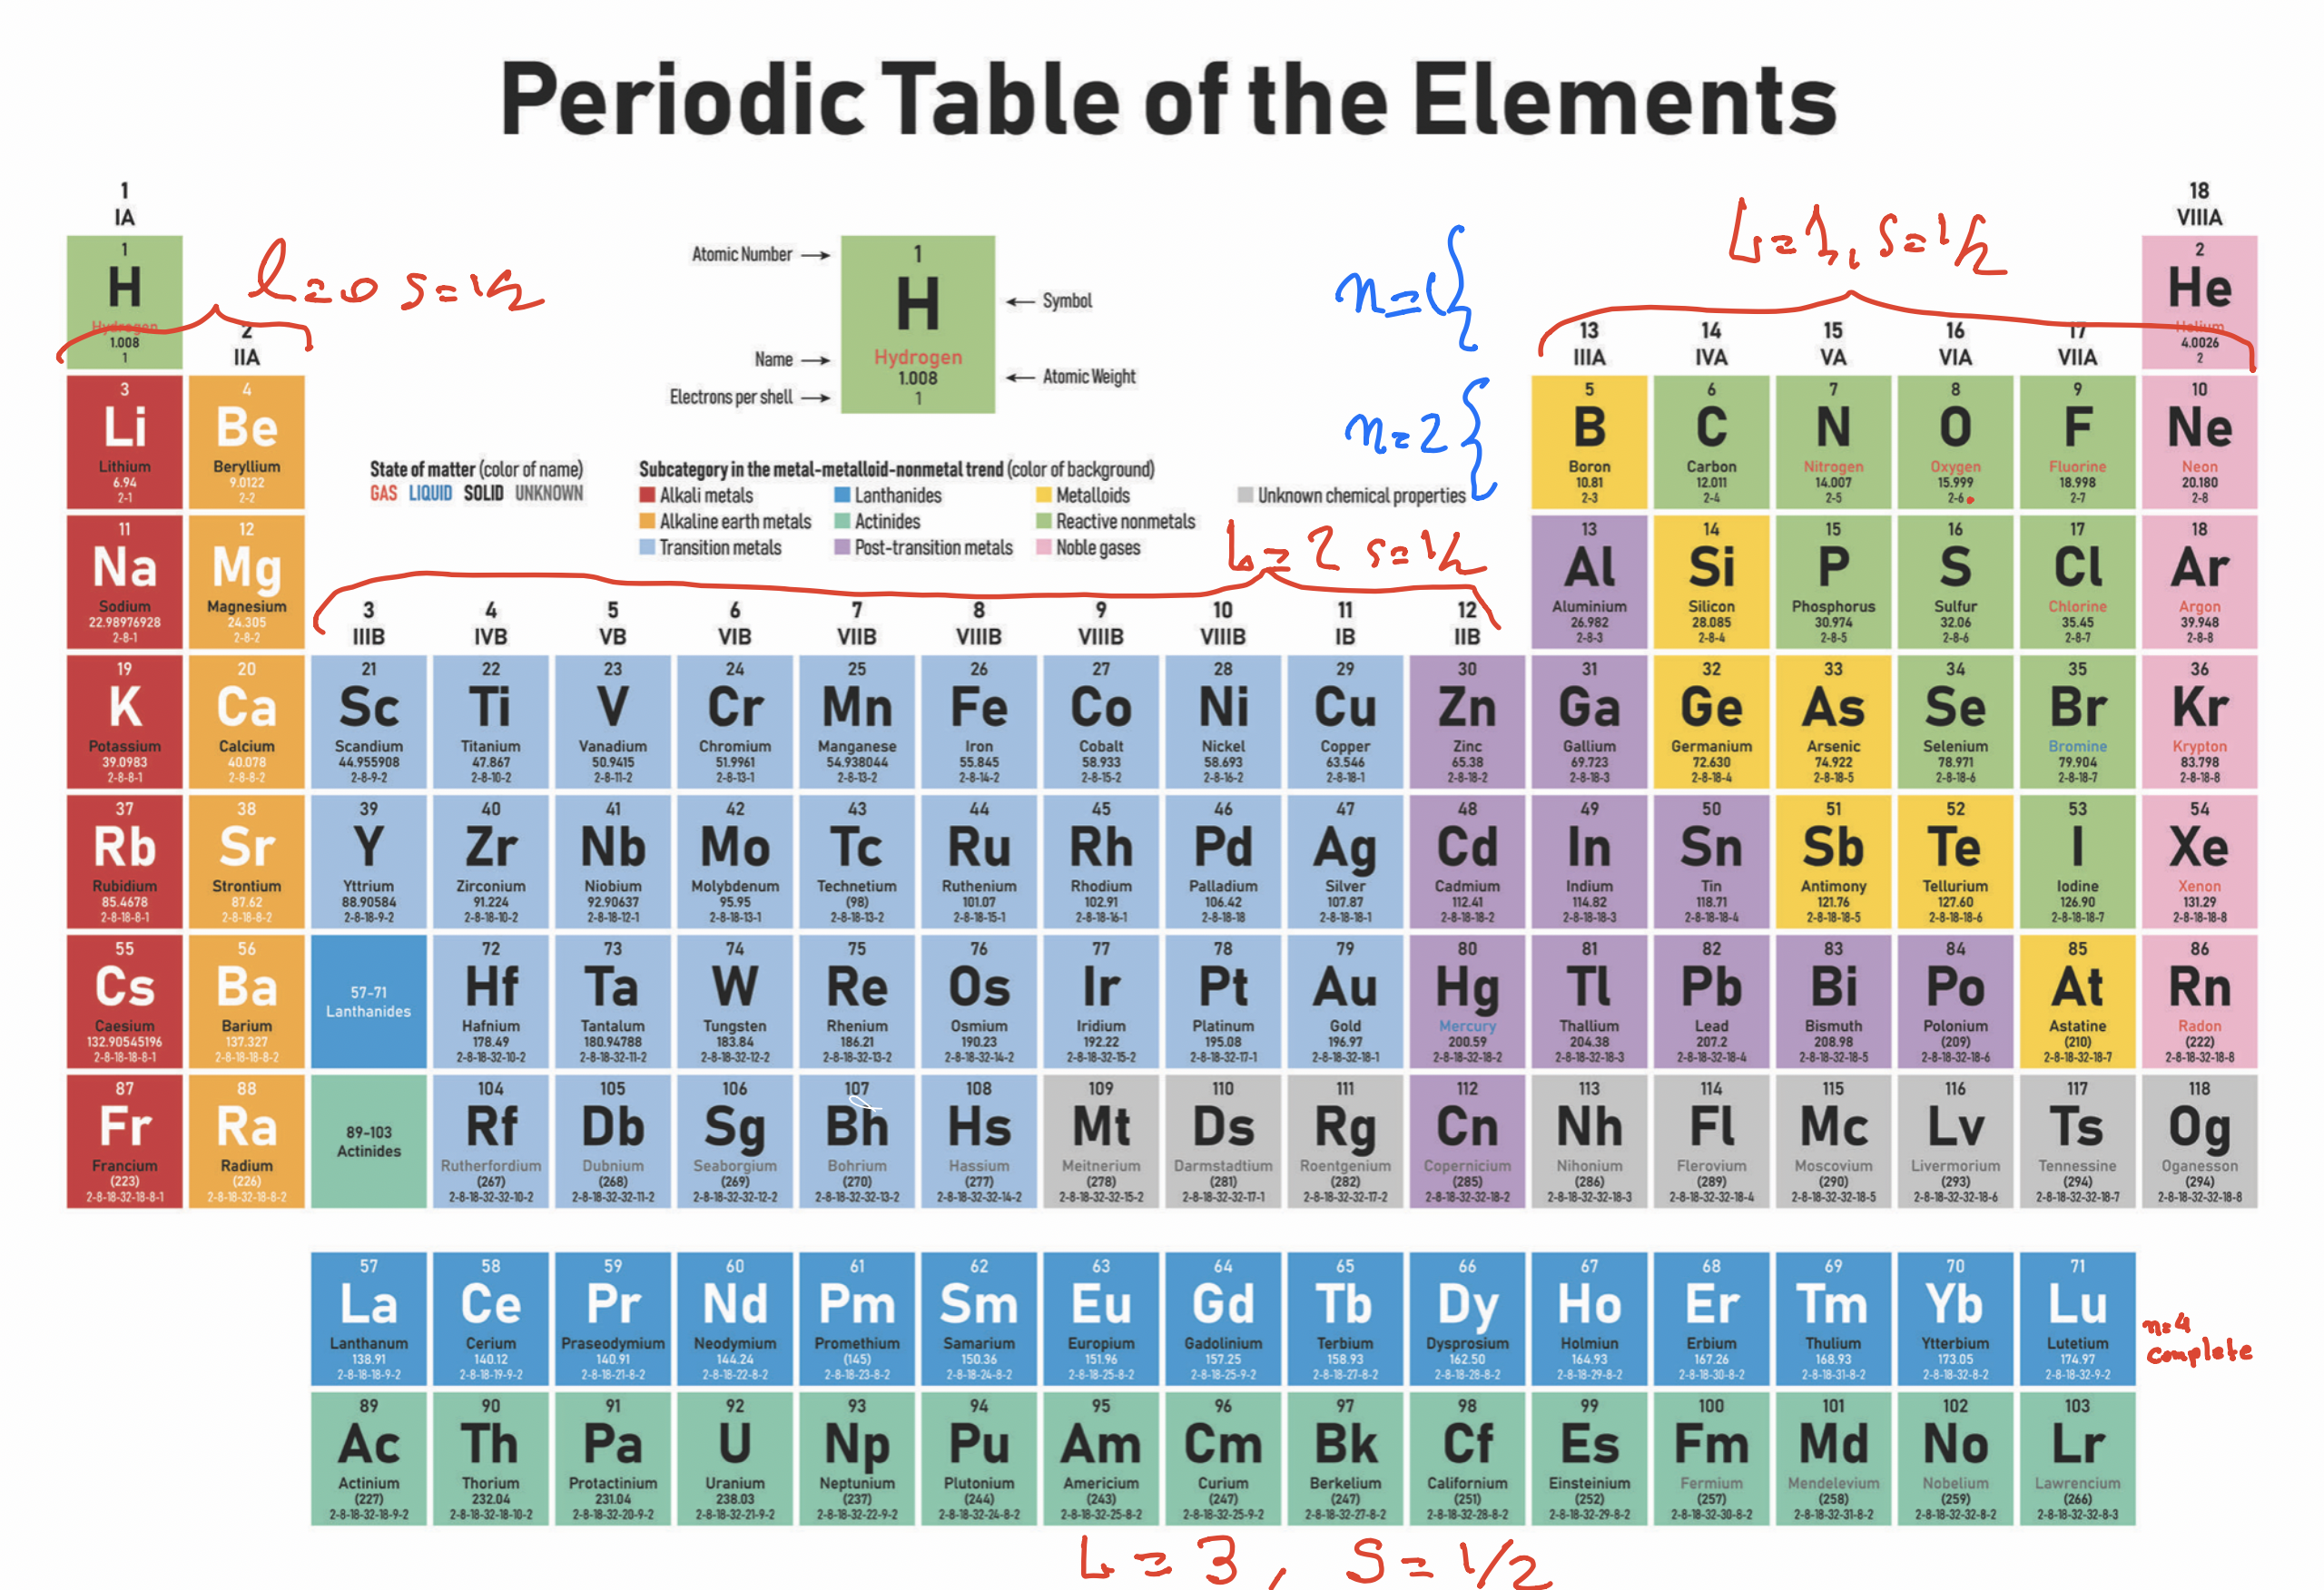
\includegraphics[width=0.7\linewidth]{periodicTable.png}
        \caption{Higher quantum states and the periodic table.}
        \label{fig:periodicTable}
    \end{figure}
    \begin{itemize}
        \item This is why the second row has the 8 states.
        \item But third row you think 18, but only 8 due to the interaction/shielding of the electrons.
        \item And then in fourth you get the 10 states there
        \item And then we get the additional states with the bottom bar (lanthanides and actinides).
        \item So we see a great interaction between spin quantum numbers and experimental periodic trends.
        \item Surprisingly and amazingly, the periodic table was constructed before quantum mechanics! We will discuss this more in three weeks.
    \end{itemize}
    \item Last thing for today: What happens if we separate the spin \emph{and} the position in the wave function as follows?
    \begin{equation*}
        \psi(\vec{r}_1,\vec{s}_1,\vec{r}_2,\vec{s}_2) = \left[ \psi_1(\vec{r}_1)\psi_2(\vec{r}_2)-\psi_1(\vec{r}_2)\psi_2(\vec{r}_1) \right]\left[
            \begin{pmatrix}
                1\\
                0\\
            \end{pmatrix}_1
            \begin{pmatrix}
                0\\
                1\\
            \end{pmatrix}_2
            -
            \begin{pmatrix}
                1\\
                0\\
            \end{pmatrix}_2
            \begin{pmatrix}
                0\\
                1\\
            \end{pmatrix}_1
        \right]
    \end{equation*}
    \begin{itemize}
        \item First off, note that there should be a $1/\sqrt{2}$ or something in there to normalize the wave function, so we're gonna talk about it as if it's normalized.
        \item What does this equation tell us?
        \item Well, imagine that $\psi_1$ is a wave packet localized somewhere in the universe, and $\psi_2$ is localized somewhere else.
        \begin{itemize}
            \item These two wave packets would have been constructed together somewhere, but they have since moved apart.
            \item This can happen with quantum particles of any spin $s$.
        \end{itemize}
        \item Takeaway: If we measure particle 1 with spin up, then particle 2 should have spin down and vice versa.
        \item We can measure such opposite spins via Stern-Gerlach experiments at different locations.
        \item Before we take a measurement, the wave function doesn't tell us anything.
        \begin{itemize}
            \item In fact, the particles have an equal probability of being spin up or spin down before measurement.
            \item However, as soon as we take a measurement of one, the state of the other snaps to the opposite of whatever we find in the original.
        \end{itemize}
        \item This is the so-called \textbf{spooky action at a distance}.
        \item You can measure in any order and in different reference frames; same result.
        \item Such systems are called \textbf{entangled states}.
    \end{itemize}
    \item \textbf{Entangled states}: Two states with some correlation of information between the properties of first and second.
    \begin{itemize}
        \item We will play with these more next quarter.
    \end{itemize}
\end{itemize}




\end{document}